This chapter explores the concept of retroactive call subsumption (RCS). RCS
enables full sharing of answers among subgoal calls, independent of the order they are called,
using the relation of subsumption.

First, we introduce the motivations behind RCS by illustrating the shortcomings of traditional call
subsumption mechanisms. Next, we present the concepts introduced by RCS and how execution
rules are extended to support retroactive tabling. Other extensions are then discussed, namely:
the new table space organization based around the ideas of the \textit{common global trie} proposal
\cite{CostaJ-08} and the algorithm to traverse the call trie to search for subsumed subgoals. Finally, we
give some details about the implementation of this new extension in the YapTab system.

\section{Motivation}

In traditional call subsumption, a new call to the subgoal $G$ is considered to create a producer subgoal
when a more general subgoal $G'$ is not found on the call trie and it is the first time $G$ is called.
When $G'$ exists, a new consumer is stored to consume answers from the subsuming subgoal $G'$, thus creating
a consumer subgoal.

Consider that subgoal \texttt{p(X,1,2)} is called first, followed by \texttt{p(X,1,Z)}.
Notice that when \texttt{p(X,1,2)} is called it is considered a producer subgoal as no subsuming subgoals
are found on the call trie. The subgoal \texttt{p(X,1,Z)} is also considered as a producer, because
\texttt{p(X,1,2)} does not subsume \texttt{p(X,1,Z)}. If the call order is swapped, \texttt{p(X,1,Z)} continues
to be considered a producer subgoal, but now \texttt{p(X,1,2)} finds \texttt{p(X,1,Z)} as a subsuming subgoal
on the call trie, and thus is considered a consumer subgoal.

While call subsumption provides good results in terms of memory utilization and time it suffers from a
major problem: the order in which the the subgoals are called can greatly affect the performance
and applicability of the technique. Therefore, we introduce a new mechanism called \textit{retroactive call
subsumption} (RCS) that solves the problem by retroactively modifying active tabled nodes to enable full sharing
of answers between subsuming and subsumed subgoals, independently of the order they are called.

\section{General Idea}

Retroactive Call Subsumption is based around the idea of stopping the computation of subsumed subgoals
that are currently running by transforming those producer subgoals into consumer subgoals, thus instead
of generating their own answers by means of code execution, they will consume answers from the more general
subgoal that has been called.

When the producer subgoal $G$ executes, an arbitrary number of choice points are created that are directly related
to $G$, that is, they are used to compute $G$'s answers. Therefore, when $G$
must be transformed into a consumer subgoal we must \textit{selectively prune} the parts of the computation
that are related to $G$ and transform $G$'s generator choice point in such a way that the choice point
will consume answers from the producer subgoal $G'$, instead of generating its own answers.
Pruning the computation of $G$ can thus potentially save execution time as $G$ no longer properly executes
but consumes answers from another subgoal.

Consider the program in Figure~\ref{fig:retro_program1} that uses RCS and the query goal `\texttt{a(X),~p(Y,Z)}'.
The goal \texttt{a(X)} starts by calling \texttt{p(1,X)}, which succeeds with the answer \texttt{\{X~=~3\}}.
By forward execution, \texttt{p(Y,Z)} is called and verifies if any subsumed subgoal is currently running
and needs to be pruned (Figure \ref{fig:retro_eval1}~(a)). It finds \texttt{p(1,X)} and thus it marks this subgoal frame as a consumer subgoal
frame that will consume from \texttt{p(Y,Z)}.
In order for \texttt{p(1,X)} to act as a consumer, its generator choice point is transformed into
a \textit{retroactive choice point}, which amounts to update the \textit{continuation alternative}
(\texttt{CP\_AP} choice point field) to an instruction called \textit{retroactive\_resolution},
which implements the needed mechanisms to control the evaluation of a \textit{retroactive node}
(Figure \ref{fig:retro_eval1}~(b)).

\begin{figure}[ht]
\begin{Verbatim}
:- use_retroactive_tabling p/2.

a(X) :- p(1, X).

p(1, 3).
p(2, 3).
p(1, 2).
\end{Verbatim}
\caption{Example program using retroactive tabling.}
\label{fig:retro_program1}
\end{figure}

Next, \texttt{p(Y,Z)} continues execution and a new answer is generated, \texttt{\{Y~=~1,~Z~=~3\}}.
By means of backtracking, all answers for \texttt{p(Y,Z)} are generated and the subgoal finally completes.
Execution returns to the retroactive choice point of \texttt{p(1,X)} and retroactive resolution is employed.
As the producer subgoal, \texttt{p(Y,Z)} has already completed, \texttt{p(1,X)} can be turned into a loader
node to consume all answers relevant to the subgoal that were not generated when the subgoal was a generator.
In this case, the only answer available is \texttt{\{X~=~2\}} (Figure \ref{fig:retro_eval1}~(c)).
Note that a retroactive node can be transformed into other types of nodes, as it will become clear in the next
sections.

\begin{figure}[ht]
  \centering
    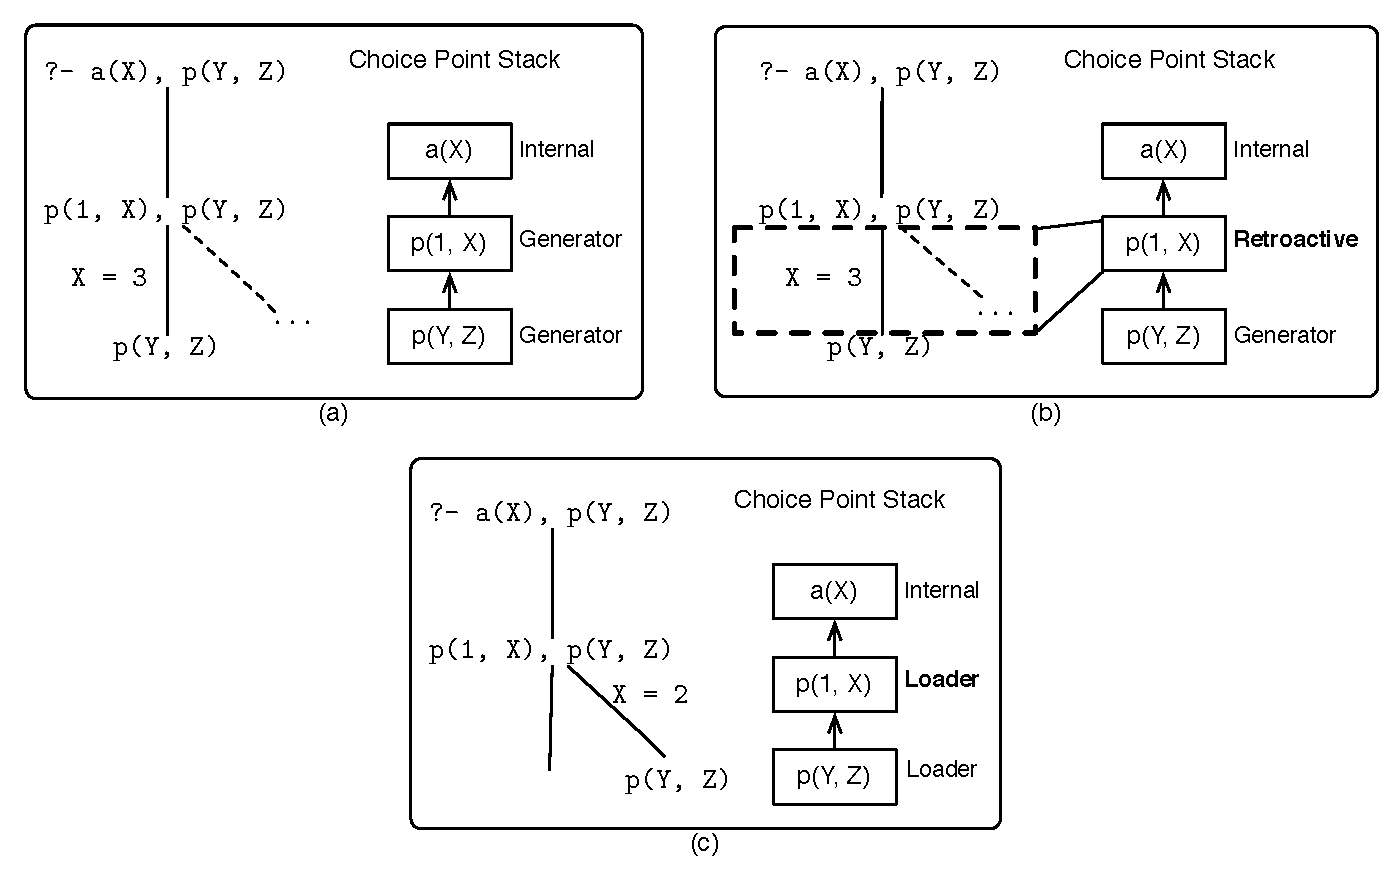
\includegraphics[scale=0.6]{pruning_example1.pdf}
  \caption{Evaluating `\texttt{a(X),~p(Y,Z)}' using retroactive tabling.}
  \label{fig:retro_eval1}
\end{figure}

The previous example has illustrated one special type of pruning called \textit{external pruning}.
External pruning occurs when the subsuming subgoal $G'$ is an \textit{external subgoal} to the evaluation
of the subsumed subgoal $G$. Another type of pruning is called \textit{internal pruning} and happens
when $G'$ is an \textit{internal subgoal} to the evaluation of $G$, that is, $G'$ is called
during the resolution of $G$. Although these two basic types of pruning can derive any other
situation, they both generate the same issues related to evaluation pruning. These issues will be explored
in detail in the next section.

\section{Pruning: Rules and Issues}

When pruning parts of the computation, we must know the areas of the local stack
that contain the choice points to prune. Given the nature of the tabling evaluation, choice points not
directly related to the pruned subgoal can get mixed with other choice points. This happens when a branch
containing external choice points has been suspended, but after backtracking to internal choice points we
execute a subsuming subgoal. Therefore, we must have a mechanism that can tell us if a certain choice
point is internal to a subgoal, from a range of choice points that can potentially contain choice points from
the pruned subgoal.

For this, we construct a dependency tree of subgoals and dependency frames by storing in a field
called \texttt{top\_gen} a pointer to the top tabled subgoal. Thus, by traversing this field we know
what subgoals the target subgoal or consumer is internal to.

When pruning execution branches, issues arise mostly when the computation of the subsumed subgoal involves
consumer and/or generators nodes. The next example programs will illustrate these issues.

Consider the program in Figure~\ref{fig:retro_program2} that mixes tabled predicates using retroactive
call subsumption and tabled predicates with variant checks.
For this program, we will use the query goal `\texttt{a(X,Y),~p(Z,W)}'.

\begin{figure}[ht]
\begin{Verbatim}
:- use_variant_tabling [a/2, b/1].
:- use_retroactive_tabling p/2.

a(X, Y) :- p(1, X), b(Y).
a(3, 4).

b(1).
b(2).

p(1, X) :- a(_, X).
p(1, X) :- b(X).
\end{Verbatim}
\caption{Example program using retroactive tabling with variant tabling.}
\label{fig:retro_program2}
\end{figure}

Initially, evaluation calls \texttt{a(X,Y)} and a new generator node is stored. Next, the retroactive subgoal
\texttt{p(1,X)} is called and creates a new generator node, because no subsuming subgoal is found.
The first clause of \texttt{p/2} executes \texttt{a(\_,X)}, which is a consumer of \texttt{a(X,Y)}, but, as
no answers are available to consume, execution suspends this node and backtracks to try to second clause
of \texttt{p/2}. Here, \texttt{b(X)} is called for the first time, creating a new generator choice point.
An answer for \texttt{b(X)} is generated, \texttt{\{X~=~1\}}, and by forward execution it is also an answer
for \texttt{p(1,X)}. Next, \texttt{b(Y)} is called, creating a new consumer node that consumes the answer
\texttt{\{X~=~1\}} and by forward execution, the first answer for \texttt{a(X,Y)}, \texttt{\{X~=~1,~Y~=~1\}},
is generated.

\begin{figure}[ht]
  \centering
    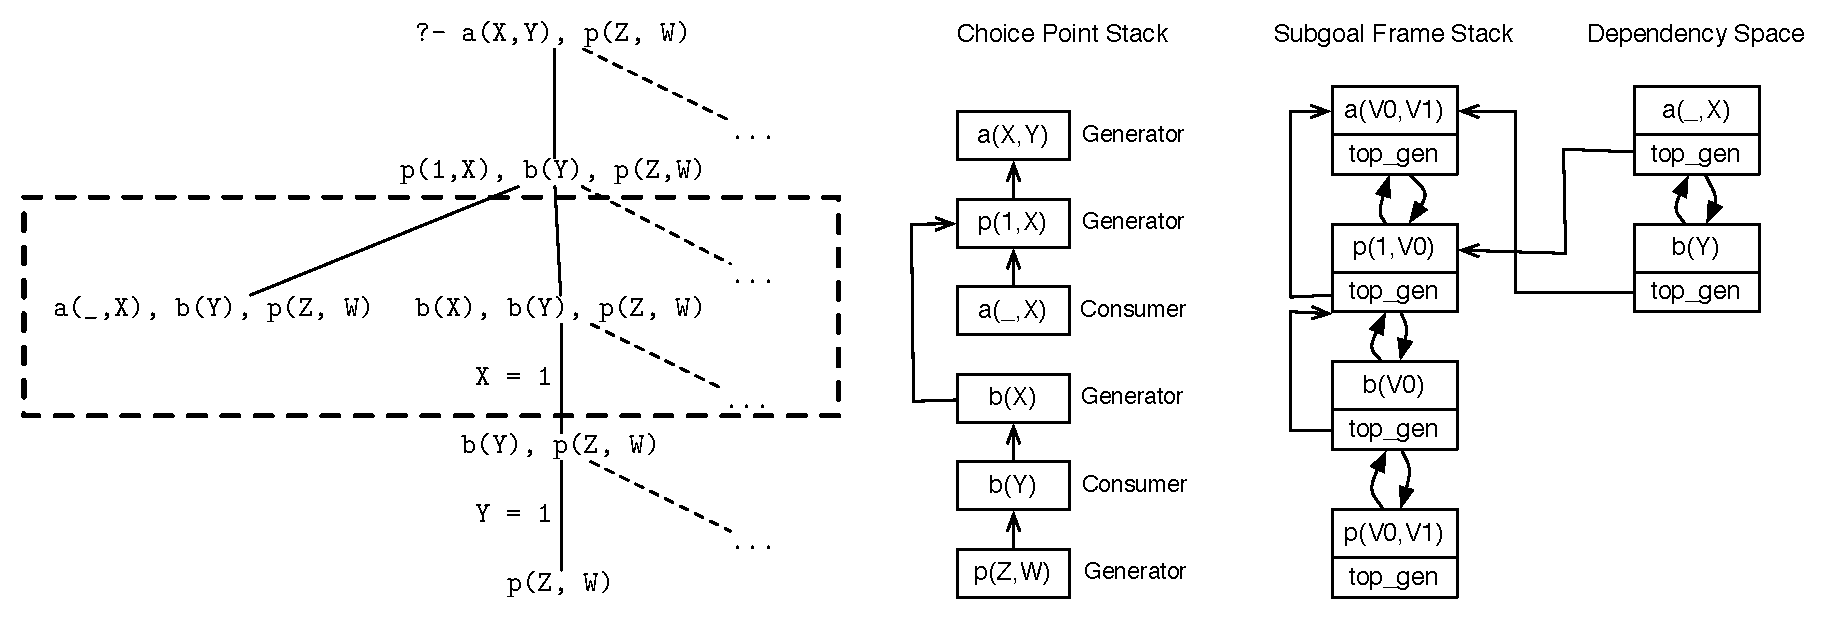
\includegraphics[scale=0.5]{retro_example2.pdf}
  \caption{Evaluating `\texttt{a(X,Y),~p(Z,W)}' using retroactive tabling.}
  \label{fig:retro_eval2}
\end{figure}

Next, subgoal \texttt{p(Z,W)} is called, which subsumes \texttt{p(1,X)} and the evaluation of this subgoal
must be pruned. Now, the subgoal \texttt{p(1,X)} includes various choice points involved in its computation,
namely \texttt{a(\_,X)} and \texttt{b(X)}.

The consumer node associated with the subgoal \texttt{a(\_,X)} must leave the computation and no longer
participates in answer resolution, thus its dependency frame is removed from the dependency space.

Pruning the generator node associated with the subgoal \texttt{b(X)} is a more tricky case. Notice that
the consumer \texttt{b(Y)} depends on this subgoal to consume new answers, thus by removing the generator node
the consumer will become an \textit{orphaned consumer} and the computation will complete too early.
Therefore, we mark the subgoal \texttt{b(X)} as \textit{pruned} and turn the consumer node of \texttt{b(Y)}
into a retroactive node.

Next, the subgoal \texttt{p(Z,W)} starts to execute the first clause of \texttt{p/2} and creates
a new consumer for \texttt{a(\_,X)}, that will consume one answer. By forward execution, an answer
for \texttt{p(Z,W)}, \texttt{\{Z~=~1,~W~=~1\}}, is generated. By means of backtracking, the second
clause of \texttt{p/2} is executed and calls \texttt{b(Y)}; as \texttt{b(Y)} is a pruned subgoal,
we first load the answers already generated for this subgoal and then execute the clauses of \texttt{b/1}.
After \texttt{b(Y)} generates all the answers, it completes successfully and execution backtracks to
\texttt{p(Z,W)}, to attempt completion of this subgoal. As the leader node is currently \texttt{a(X,Y)},
completion fails.

We backtrack to the retroactive node \texttt{b(Y)} will order to do retroactive resolution. Evaluation
notices that the subgoal has already completed, thus the retroactive node is transformed into a loader node
to consume all answers that were not consumed. By forward execution, a new consumer for \texttt{p(Z,W)} is
created that will generate more answers for the query goal. Once \texttt{b(Y)} does not have more answers
to consume, execution backtracks to the retroactive node of \texttt{p(1,X)}. Here, we note that
the producer subgoal, \texttt{p(Z,W)} has still not completed and this retroactive node must be turned
into a consumer node, which amounts to create a new dependency frame that is added into the dependency space,
in order to participate in the resolution process.

After \texttt{p(1,X)} executes the answer resolution
operation, evaluation backtracks to \texttt{a(X,Y)} that will execute the second clause of \texttt{a/2}.
Once \texttt{a(X,Y)} executes the completion operation and each each consumer has consumed its answers,
the subgoal completes and evaluation is finished.

\subsection{Pruning Actions}

The previous example has illustrated the different actions that must be applied to each choice point that
makes part of the computation of the subsumed subgoal. This action is dependent on the choice point
type and is summarized in the next subsections.

\subsubsection{Interior Nodes}

Interior nodes are related to normal Prolog execution and can be easily pruned
by ignoring them altogether. This approach, while simple, suffers from the problem of \textit{trapped
choice points}. This problem also affects delaying based tabling engines like YapTab and SLG-WAM, where
choice points under consumers are frozen and remain until completion. The CHAT approach to tabling
solves this problem by removing trapped choice points \cite{Demoen-99b}. Another solution would involve
modifications to the WAM garbage collector to collect unused space on the choice point stack.


\subsubsection{Internal Consumers}   
   
Internal consumers must be explicitly pruned by removing the associated
dependency frame from the dependency space. Thus prevents the resolution process to reactivate pruned
branches. In the previous example, \texttt{a(\_,X)} was an internal consumer.

\begin{figure}[ht]
\begin{Verbatim}
abolish_dependency_frames(specific_sg, min, max) {
   top = dependency_frame_before(specific_sg, max)

   while (top != NULL and younger_than(depfr_cons_cp(top), min))
      depfr = top
      top = depfr_next(depfr)

      if (is_internal_depfr(specific_sg, depfr, min))
         remove_from_stack(depfr)
         free(dep_fr)
}
\end{Verbatim}
\caption{Pseudo-code for procedure \texttt{abolish\_dependency\_frames}.}
\label{fig:abolish_dependency_frames}
\end{figure}
   
Figure~\ref{fig:abolish_dependency_frames} shows the procedure that abolishes internal dependency frames.
The arguments are: \texttt{specific\_sg}, the subsumed subgoal to prune; \texttt{min}, the first choice point address from the range of choice points to selectively prune; and \texttt{max}, the last choice point from the pruned range. First, we compute the first dependency frame inside the choice point range by using the function \texttt{dependency\_frame\_before}. Next, we iterate the dependency frames inside the range and check if they are internal to the choice point; if they are, we remove them from the dependency space.

\subsubsection{Internal Generators}

For internal generators we must remove its corresponding subgoal frame
from the subgoal frames stack and alter its state to pruned. Generally, when pruning internal generators, we
have two situations: (1) the generator does not have consumers that are external to the computation of the
subsumed subgoal; or (2) the generator has external consumers. The former situation does not introduce any
problem, but the latter origins orphaned consumers. In our example, the consumer node for \texttt{b(Y)} is
an orphaned consumer.

Usually, a pruned generator is called again during the evaluation of the subsuming subgoal, and before
the computation reaches any of the orphaned consumers. Once reactivated, the subgoal frame for the pruned
generator is pushed again into the top of the subgoal frame stack and its state is altered to
\textit{evaluating}. Then, the new generator node starts by consuming the previously generated answers
and only then executes the program clauses.

\begin{figure}[ht]
\begin{Verbatim}
abolish_subgoal_frames(specific_sg, min, max) {
   top = subgoal_frame_before(specific_sg, max)

   while (top != NULL and younger_or_equal(generator_cp(top), min))
      sg_fr = top
      top = next(sg_fr)

      if (is_internal_subgoal_frame(specific_sg, sg_fr, min))
         sg_cp = generator_cp(sg_fr)
         
         remove_subgoal_from_stack(sg_fr)
         
         if (type(sg_fr) == VARIANT or type(sg_fr) == RETROACTIVE)
            if (has_external_consumers(sg_fr))
               update_external_consumers(specific_sg, sg_fr, sg_cp, max)
               state(sg_fr) = pruned
            else
               free(sg_fr)
         else if (type(sg_fr) == SUBSUMPTIVE)
            if (has_proper_consumers(sg_fr))
               transform_external_subsumed_consumers(specific_sg, sg_fr, sg_cp, max)
            
            if (has_variant_consumers(sg_fr))
               update_external_consumers(specific_sg, sg_fr, sg_cp, max)
               
            if (has_no_consumers(sg_fr))
               free(sg_fr)
}
\end{Verbatim}
\caption{Pseudo-code for procedure \texttt{abolish\_subgoal\_frames}.}
\label{fig:abolish_subgoal_frames}
\end{figure}


\subsection{Orphaned Consumers}

\subsection{Lost Consumers}

\subsection{Frontier Choice Point}

\subsection{Leader Re-Computation}

\section{Internal Pruning}

\section{Mixing External and Internal Pruning}

\section{Table Space}

\section{Searching Subsumed Subgoals}

\section{Implementation Details}

\subsection{Retroactive Resolution}

\subsection{Subgoal Frames}

\subsection{External or Internal}

\subsection{Transforming Consumers Into Generators}

\subsection{Subgoal Dependency Tree}

\subsection{Reference Counting}